% TITLE:
% Author: Adrian Schrader
% Created on: 31/7/15

\documentclass[a4paper, 10pt, twocolumn]{scrartcl}
\usepackage[ngerman]{babel}

% Mathematics
\usepackage{amsmath}
\usepackage{amssymb}
\numberwithin{equation}{subsection}

% Font and Style
\usepackage{ucs}
\usepackage[T1]{fontenc}
\usepackage{abstract}
\usepackage{url}
\usepackage{lipsum}
\usepackage{hyperref}
\hypersetup{colorlinks=false}

% Font Package (select one)
%\usepackage{lmodern}
%\usepackage{kpfonts}
%\usepackage{ccfonts}
\usepackage{cmbright}
%\usepackage{antpolt}
%\usepackage{iwona}

% Bibliography
\usepackage[numbers,round]{natbib}
\usepackage[babel,german=guillemets]{csquotes}
\bibliographystyle{alphadin}

% Image and Graphics
\usepackage{graphicx}
\usepackage{dblfloatfix}
\usepackage[left=2.5cm, right=2.5cm, top=2.5cm, bottom=3cm]{geometry}
\setlength{\columnsep}{15pt}

% Source Code
\usepackage{caption}
\usepackage[section]{minted}
\usemintedstyle{trac}
\setminted[java]{
  autogobble,
  mathescape,
  fontfamily=courier,
  breaklines,
  fontsize=\footnotesize,
  framesep=2mm,
  baselinestretch=1.2}
\renewcommand{\listingscaption}{Quellcode}

% Document Information
\title{A long and complex document title}
\subtitle{Further specification goes here}
\author{Adrian Schrader}
\date{\today}

\begin{document}
  % Create Title, Abstract and TOC
  \twocolumn[\maketitle \begin{abstract} \begin{minipage}{1.0\linewidth}
    \input{tex/abstract}
  \vspace{0.8cm} \end{minipage}\end{abstract}]
  \tableofcontents

  % CONTENT
  % TITLE: Lipsum text with two figures and math
% AUTHOR: Adrian Schrader
% Created on: 31/7/15

\section{Normal figures}
\lipsum[1-2]\footnote{This is an unnecessary footnote. Thanks!}

\begin{figure}[h]
  \centering
  \includegraphics[width=\linewidth]{img/plot}
  \caption{Plot of of f(t) in maple}
  \label{img:function}
\end{figure}

\lipsum[3-4]

\subsection{Page wide figures}
\lipsum[5]

\begin{figure*}[ht]
  \centering
  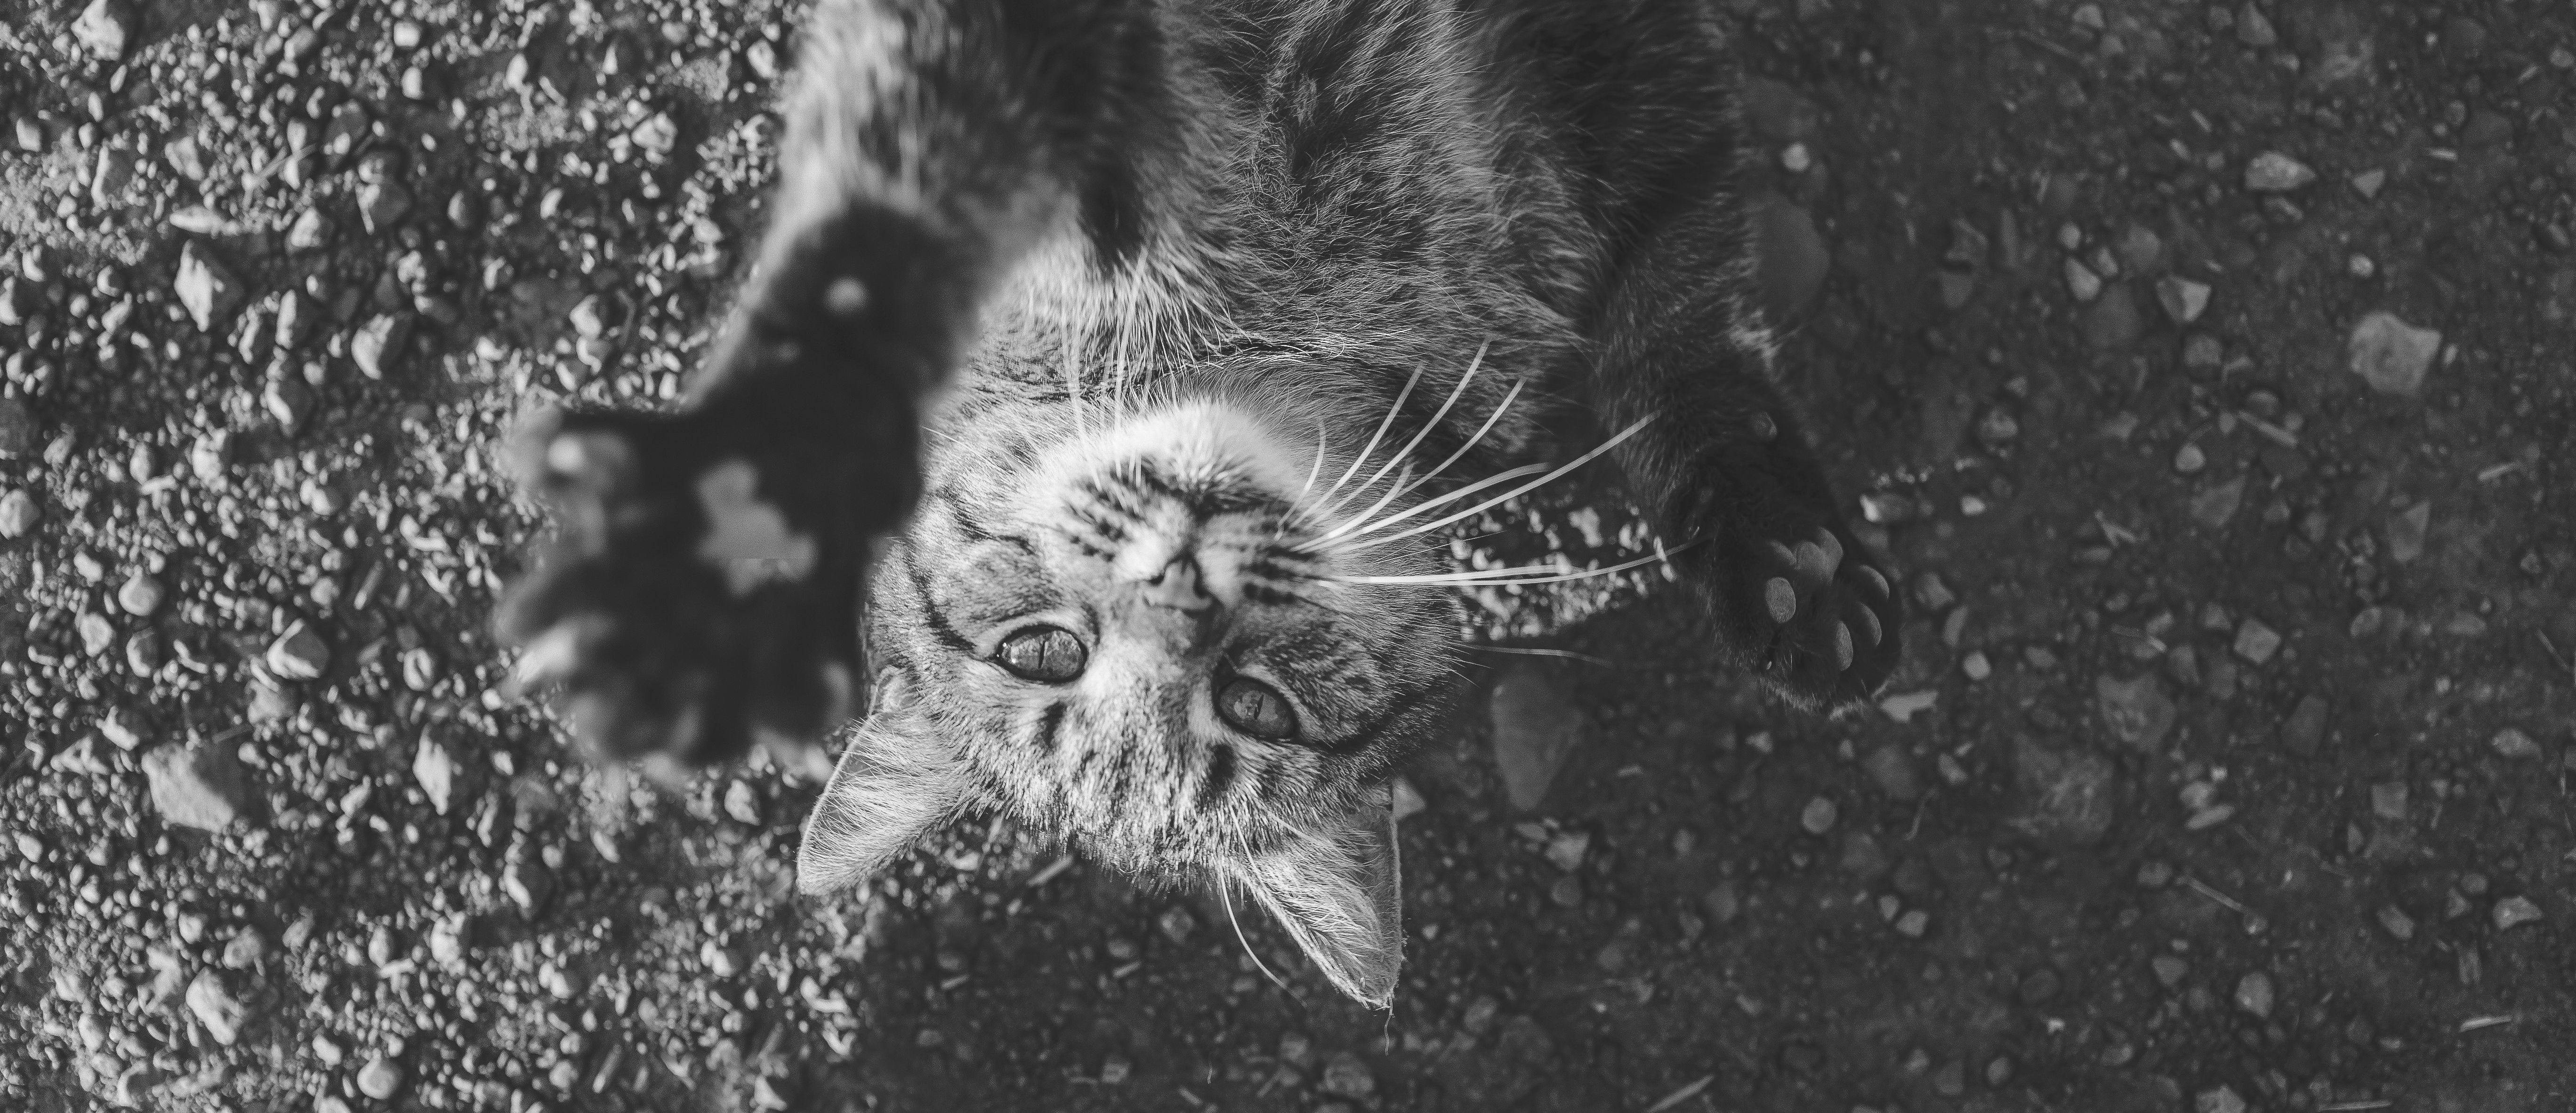
\includegraphics[width=\linewidth]{img/example2}
  \caption{Another Random cat picture from Google \protect\url{https://static.pexels.com/photos/4067/animal-pet-cute-cat.jpg}}
  \label{img:cat2}
\end{figure*}

\subsection{Formulas and plots}
\lipsum[6]
\begin{figure}[h]
  \centering
  \includegraphics[width=\linewidth]{img/spectrum}
  \caption{Plot of the spectrum of f(t) in maple}
  \label{img:spectrum}
\end{figure}

\begin{align}
    f(t) &= s_0 \cdot e^{-\frac{t}{\tau}} \cdot cos(\omega_s t) \cdot \Theta(t) \nonumber \\
    &= s_0 \cdot e^{-\frac{t}{\tau}} \cdot \frac{1}{2} \Big( e^{i \omega_s t} + e^{-i \omega_s t} \Big) \cdot \Theta(t)\\
    \tilde{f}(\omega) &= \mathcal{F}(f)(\omega) = \frac{1}{\sqrt{2\pi}} \int_{-\infty}^{\infty} f(t) \cdot e^{-i \omega t} dt \nonumber\\
    &= \frac{s_0}{\sqrt{2\pi}} \frac{\frac{1}{\tau} + i \omega}{(\frac{1}{\tau} + i \omega)^2 + \omega_s^2}
\end{align}

\section{Source codes}
\begin{listing}
  \begin{minted}{java}
    public static void main(String[] args) {
      return;
    }
  \end{minted}
  \caption{Standard main method of every java program}
  \label{lst:javamain}
\end{listing}

\lipsum[9-12]

\subsection{Subsection Two.One}
\lipsum[13-14]


  % Bibliography
  \bibliography{bib/bibliography.bib}
\end{document}
